% ============================================================
% M2 轮4 S3 · 练习件 第2课时（§1.1.1 课2 空间向量的数量积）
% 题面：照题面库 成卷/题面库/课时02-1.1.1课2.md 全 16 题冻结入卷（卷面题号＝库序 1~16）；
%       组名/难度照库头第 3/4 字段（第14题 难度简单→升中档，定稿A 偏差注记）。
% 模板基线＝练习线样张（六宏零改动拷入）；版式＝练习线 p2 课时训练
%       （\keshi＋multicols＋花形三档 基础巩固1~10／综合提升11~14／思维探索15~16）。
% 图源：第4题＝单元2/word/media/image5.png → figs/dy2_image5.png（28mm，题干后）。
% 取值/组名照登对照/图位/登记事项：见 ../批1值台账.md 课时02 节。
% 编译：xelatex main.tex（两遍）→ python render.py → png/pageN.png
% ============================================================
\documentclass[fontset=none]{ctexart}
\usepackage{qp-m3} % 换装：六宏→qp-m3 单包（钉后版 md5 7c3930362be8a0a2bdf21bbf8ac16573，两补钉随版）

% ============================================================
% 练习件局部宏（照练习线样张页2形制搬入；本段只加件，不改件）
% ============================================================
\renewcommand{\qpjianming}{练习件}
\renewcommand{\qpceming}{高中数学\quad 选择性必修第一册(人教B版)} % 换装回钉：qp-m3 默认册名＝选必二，防页脚漂移（试迁规约·试迁报告§四 B3 实证必改）
\renewcommand{\qpzhangming}{第一章\quad 空间向量与立体几何}

% ---------- YJ-01 灰块页脚·练习册档（块 31.0×7.8mm，照练习线样张 31.0mm 修正版） ----------
\newcommand{\qpxsyema}{\ifnum\value{page}<10 00\fi\ifnum\value{page}>9 \ifnum\value{page}<100 0\fi\fi\arabic{page}}
\newcommand{\lxshuziL}{\hbox to 13.8mm{\setlength{\fboxsep}{0pt}\colorbox{pnumbg}{%
  \makebox[31.0mm][l]{\rule[-3.145mm]{0pt}{7.8mm}\hspace{2.8mm}\fontsize{10.7pt}{13pt}\selectfont\color{black}\numpnum\qpxsyema}}\hss}}
\newcommand{\lxshuziR}{\hbox to 13.8mm{\kern-17.2mm\setlength{\fboxsep}{0pt}\colorbox{pnumbg}{%
  \makebox[31.0mm][r]{\rule[-3.145mm]{0pt}{7.8mm}\fontsize{10.7pt}{13pt}\selectfont\color{black}\numpnum\qpxsyema\hspace{2.75mm}}}}}
\fancyfoot[RO]{\raisebox{-1.24mm}[0pt][0pt]{\qphuitext\qpzhangming\quad{\heiti\qpjianming}\hspace{3mm}\lxshuziL}}
\fancyfoot[LE]{\raisebox{-1.24mm}[0pt][0pt]{\lxshuziR\hspace{3mm}\qphuitext\qpceming}}

% ---------- HX-01 花形·三档名（练习册版 25.5×6.8mm，重叠 o＝5.1mm） ----------
% 局部宏 \huadianOverlapLx 已由 qp-m3 收编（等值定义），依换装方案§1.4 预删防撞名
% 局部宏 \dangbadge 已由 qp-m3 收编（等值定义），依换装方案§1.4 预删防撞名

% ---------- TJ-02 练习册悬挂题号（单号 5.75mm／双位 7.6mm） ----------
% 长度 \lxhang 已由 qp-m3 分配，预删防重复定义
% 局部宏 \tihao 已由 qp-m3 收编（等值定义），依换装方案§1.4 预删防撞名
% 局部宏 \lxopt 已由 qp-m3 收编（等值定义），依换装方案§1.4 预删防撞名
% 局部宏 \xiexwei 已由 qp-m3 收编（等值定义），依换装方案§1.4 预删防撞名
% 局部宏 \zu 已由 qp-m3 收编（等值定义），依换装方案§1.4 预删防撞名

\begin{document}
%成书重装五本跨本连续页码（G7方案B，承M2/M3装配先例）setcounter 注入位
\setcounter{page}{43}

% ============================================================
% 课时训练（三档 10＋4＋2＝16 题）
% ============================================================
\keshi{第2课时\quad 空间向量的数量积}
\begin{multicols}{2}
\emergencystretch=1em

\dangbadge{基}{础}{巩}{固}

\tihao{1}\zu{W1 空间向量概念×五命题计数选型} \tieside{简单}下列关于空间向量的命题中，正确命题的个数是\nobreak(\kongwei)
\lxopt{①任一向量与它的相反向量都不相等；}
\lxopt{②长度相等、方向相同的两个向量是相等向量；}
\lxopt{③平行且模相等的两个向量是相等向量；}
\lxopt{④若\(\overrightarrow{a}\neq\overrightarrow{b}\)，则\(|\overrightarrow{a}|\neq|\overrightarrow{b}|\)；}
\lxopt{⑤两个向量相等，则它们的起点与终点相同．}
\lxopt{\makebox[\dimexpr0.25\linewidth-0.5em\relax][l]{A．0；}\makebox[\dimexpr0.25\linewidth-0.5em\relax][l]{B．1；}\makebox[\dimexpr0.25\linewidth-0.5em\relax][l]{C．2；}\makebox[\dimexpr0.25\linewidth-0.5em\relax][l]{D．3}}
\begin{ansblock}[练-课时02-1]
% ans:练-课时02-1
\ansitem{1}{B（仅②真）}
\end{ansblock}

\tihao{2}\zu{W3 正方体线性运算×化简定向选型} \tieside{简单}在正方体\(ABCD\text{-}\penalty100 A_1B_1C_1D_1\)中，下列各式的运算结果为向量\(\overrightarrow{B_1D_1}\)的是\nobreak(\kongwei)
\lxopt{①\(\overrightarrow{A_1D_1}-\overrightarrow{A_1A}-\overrightarrow{AB}\)；}
\lxopt{②\(\overrightarrow{BC}+\overrightarrow{BB_1}-\overrightarrow{D_1C_1}\)；}
\lxopt{③\(\overrightarrow{AD}-\overrightarrow{AB_1}+\overrightarrow{DD_1}\)；}
\lxopt{④\(\overrightarrow{B_1D_1}-\overrightarrow{AA_1}+\overrightarrow{DD_1}\)．}
\lxopt{\makebox[\dimexpr0.25\linewidth-0.5em\relax][l]{A．①②；}\makebox[\dimexpr0.25\linewidth-0.5em\relax][l]{B．②③；}\makebox[\dimexpr0.25\linewidth-0.5em\relax][l]{C．③④；}\makebox[\dimexpr0.25\linewidth-0.5em\relax][l]{D．①④}}
\begin{ansblock}[练-课时02-2]
% ans:练-课时02-2
\ansitem{2}{C（③④）}
\end{ansblock}

\tihao{3}\zu{W4 加法三角形法则×四边形形状判定} \tieside{简单}设有四边形\(ABCD\)，\(O\)为空间任意一点，且\(\overrightarrow{AO}+\overrightarrow{OB}=\overrightarrow{DO}+\overrightarrow{OC}\)，则四边形\(ABCD\)是\nobreak(\kongwei)
\lxopt{\makebox[\dimexpr0.5\linewidth-0.5\lxhang-0.25em\relax][l]{A．空间四边形；}\makebox[\dimexpr0.5\linewidth-0.5\lxhang-0.25em\relax][l]{B．平行四边形}}
\lxopt{\makebox[\dimexpr0.5\linewidth-0.5\lxhang-0.25em\relax][l]{C．等腰梯形；}\makebox[\dimexpr0.5\linewidth-0.5\lxhang-0.25em\relax][l]{D．矩形}}
\begin{ansblock}[练-课时02-3]
% ans:练-课时02-3
\ansitem{3}{B（平行四边形）}
\end{ansblock}

\tihao{4}\zu{W5 正三角形中心化简×填空} \tieside{简单}在空间四边形\(ABCD\)中，若\(\triangle BCD\)是正三角形，且\(E\)为其中心，连接\(DE\)，则\nobreak\(\overrightarrow{AB}+\frac{1}{2}\overrightarrow{BC}-\frac{3}{2}\overrightarrow{DE}-\overrightarrow{AD}\)的化简结果为\kongbai{}．
\par\vspace{1.9mm}\penalty10000\noindent\makebox[\linewidth][c]{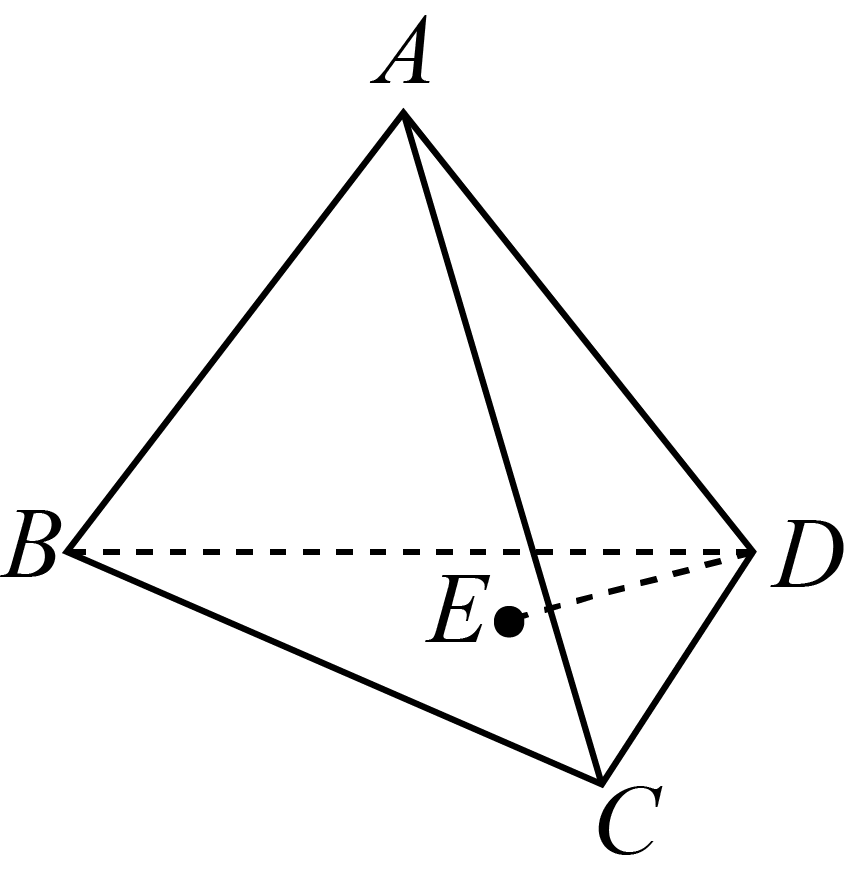
\includegraphics[width=28mm]{figs/dy2_image5.png}}\par\vspace{-1.0mm}\penalty10000
\begin{ansblock}[练-课时02-4]
% ans:练-课时02-4
\ansitem{4}{\(\overrightarrow{0}\)}
\end{ansblock}

\tihao{5}\zu{W6 给定式系数算术化简×填空} \tieside{简单}化简：\(\frac{1}{2}(\overrightarrow{a}+2\overrightarrow{b}-3\overrightarrow{c})+5[\frac{2}{3}\overrightarrow{a}-\frac{1}{2}\overrightarrow{b}+\frac{2}{3}\overrightarrow{c}]-3(\overrightarrow{a}-2\overrightarrow{b}+\overrightarrow{c})\)．
\xiexwei{16mm}
\begin{ansblock}[练-课时02-5]
% ans:练-课时02-5
\ansitem{5}{\(\dfrac{5}{6}\overrightarrow{a}+\dfrac{9}{2}\overrightarrow{b}-\dfrac{7}{6}\overrightarrow{c}\)}
\end{ansblock}

\tihao{6}\zu{W8 共面向量组判定×说理题组} \tieside{简单}在正方体\(ABCD\text{-}\penalty100 A_1B_1C_1D_1\)中，判断下列各组向量是否共面：
\lxopt{(1)\(\overrightarrow{AB}\)，\(\overrightarrow{D_1C_1}\)；}
\lxopt{(2)\(\overrightarrow{AB}\)，\(\overrightarrow{BC}\)，\(\overrightarrow{A_1D_1}\)；}
\lxopt{(3)\(\overrightarrow{AB}\)，\(\overrightarrow{BC}\)，\(\overrightarrow{DD_1}\)．}
\xiexwei{16mm}
\begin{ansblock}[练-课时02-6]
% ans:练-课时02-6
\ansitem{6}{(1)共面；(2)共面；(3)不共面}
\end{ansblock}

\tihao{7}\zu{W9 正方体向量夹角求值×题组} \tieside{简单}已知\(ABCD\text{-}\penalty100 A_1B_1C_1D_1\)是一个正方体，写出下列向量夹角的大小：
\lxopt{(1)\(\langle\overrightarrow{AB},\overrightarrow{CC_1}\rangle\)；}
\lxopt{(2)\(\langle\overrightarrow{DD_1},\overrightarrow{BA_1}\rangle\)．}
\xiexwei{16mm}
\begin{ansblock}[练-课时02-7]
% ans:练-课时02-7
\ansitem{7}{(1)\(90^{\circ}\)；(2)\(45^{\circ}\)}
\end{ansblock}

\tihao{8}\zu{W9$\langle 2a,-3b\rangle$系数换角} \tieside{简单}已知\(\overrightarrow{a}\)，\(\overrightarrow{b}\)都是空间向量，且\(\langle\overrightarrow{a},\overrightarrow{b}\rangle=\frac{\pi}{4}\)，求\(\langle 2\overrightarrow{a},-3\overrightarrow{b}\rangle\)．
\xiexwei{16mm}
\begin{ansblock}[练-课时02-8]
% ans:练-课时02-8
\ansitem{8}{\(\dfrac{3\pi}{4}\)}
\end{ansblock}

\tihao{9}\zu{W11 四棱柱基底表示 BD$_1$×单选} \tieside{简单}已知四棱柱\(ABCD\text{-}\penalty100 A_1B_1C_1D_1\)的底面\(ABCD\)是平行四边形，且\(\overrightarrow{AB}=\overrightarrow{a}\)，\(\overrightarrow{AD}=\overrightarrow{b}\)，\(\overrightarrow{AA_1}=\overrightarrow{c}\)，则\nobreak\(\overrightarrow{BD_1}=\)(\kongwei)
\lxopt{\makebox[\dimexpr0.5\linewidth-0.5\lxhang-0.25em\relax][l]{A．\(\overrightarrow{a}+\overrightarrow{b}+\overrightarrow{c}\)；}\makebox[\dimexpr0.5\linewidth-0.5\lxhang-0.25em\relax][l]{B．\(-\overrightarrow{a}+\overrightarrow{b}+\overrightarrow{c}\)}}
\lxopt{\makebox[\dimexpr0.5\linewidth-0.5\lxhang-0.25em\relax][l]{C．\(\overrightarrow{a}-\overrightarrow{b}+\overrightarrow{c}\)；}\makebox[\dimexpr0.5\linewidth-0.5\lxhang-0.25em\relax][l]{D．\(-\overrightarrow{a}+\overrightarrow{b}-\overrightarrow{c}\)}}
\begin{ansblock}[练-课时02-9]
% ans:练-课时02-9
\ansitem{9}{B（\(-\overrightarrow{a}+\overrightarrow{b}+\overrightarrow{c}\)）}
\end{ansblock}

\tihao{10}\zu{W19 共线定理三点共线判定×选型} \tieside{简单}已知向量\(\overrightarrow{a}\)，\(\overrightarrow{b}\)，且\(\overrightarrow{AB}=\overrightarrow{a}+2\overrightarrow{b}\)，\(\overrightarrow{BC}=-5\overrightarrow{a}+6\overrightarrow{b}\)，\(\overrightarrow{CD}=7\overrightarrow{a}-2\overrightarrow{b}\)，则一定共线的三点是\nobreak(\kongwei)
\lxopt{\makebox[\dimexpr0.5\linewidth-0.5\lxhang-0.25em\relax][l]{A．\(A\)，\(B\)，\(D\)；}\makebox[\dimexpr0.5\linewidth-0.5\lxhang-0.25em\relax][l]{B．\(A\)，\(B\)，\(C\)}}
\lxopt{\makebox[\dimexpr0.5\linewidth-0.5\lxhang-0.25em\relax][l]{C．\(B\)，\(C\)，\(D\)；}\makebox[\dimexpr0.5\linewidth-0.5\lxhang-0.25em\relax][l]{D．\(A\)，\(C\)，\(D\)}}
\begin{ansblock}[练-课时02-10]
% ans:练-课时02-10
\setlength{\anshang}{7.6mm}% 题10 起双位档（照答案册同值，块内局部）
\ansitem{10}{A（\(A\)、\(B\)、\(D\)）}
\end{ansblock}

\dangbadge{综}{合}{提}{升}

\tihao{11}\zu{W15 正方体底面中心 AO$_1$·AC 分解求值×单选} \tieside{中档}已知棱长为\(1\)的正方体\(ABCD\text{-}\penalty100 A_1B_1C_1D_1\)的上底面\(A_1B_1C_1D_1\)的中心为\(O_1\)，则\nobreak\(\overrightarrow{AO_1}\cdot\overrightarrow{AC}\)的值为\nobreak(\kongwei)
\lxopt{\makebox[\dimexpr0.25\linewidth-0.25\lxhang-0.25em\relax][l]{A．\(-1\)；}\makebox[\dimexpr0.25\linewidth-0.25\lxhang-0.25em\relax][l]{B．\(0\)；}\makebox[\dimexpr0.25\linewidth-0.25\lxhang-0.25em\relax][l]{C．\(1\)；}\makebox[\dimexpr0.25\linewidth-0.25\lxhang-0.25em\relax][l]{D．\(2\)}}
\begin{ansblock}[练-课时02-11]
% ans:练-课时02-11
\setlength{\anshang}{7.6mm}% 题11 起双位档（照答案册同值，块内局部）
\ansitem{11}{C（\(1\)）}
\end{ansblock}

\tihao{12}\zu{W16 正四面体对棱向量夹角×单选} \tieside{中档}若空间四边形\(OABC\)的四个面均为等边三角形，则\nobreak\(\cos\langle\overrightarrow{OA},\overrightarrow{BC}\rangle\)的值为\nobreak(\kongwei)
\lxopt{\makebox[\dimexpr0.25\linewidth-0.25\lxhang-0.25em\relax][l]{A．\(\frac{1}{2}\)；}\makebox[\dimexpr0.25\linewidth-0.25\lxhang-0.25em\relax][l]{B．\(\frac{\sqrt{2}}{2}\)；}\makebox[\dimexpr0.25\linewidth-0.25\lxhang-0.25em\relax][l]{C．\(-\frac{1}{2}\)；}\makebox[\dimexpr0.25\linewidth-0.25\lxhang-0.25em\relax][l]{D．\(0\)}}
\begin{ansblock}[练-课时02-12]
% ans:练-课时02-12
\setlength{\anshang}{7.6mm}% 题12 起双位档（照答案册同值，块内局部）
\ansitem{12}{D（\(0\)）}
\end{ansblock}

\tihao{13}\duoxuan\zu{W18 长方体数量积「可为0」存在性×多选} \tieside{中档}已知长方体\(ABCD\text{-}\penalty100 A_1B_1C_1D_1\)，则下列向量的数量积可以为\(0\)的是\nobreak(\kongwei)
\lxopt{\makebox[\dimexpr0.5\linewidth-0.5\lxhang-0.25em\relax][l]{A．\(\overrightarrow{AD_1}\cdot\overrightarrow{B_1C}\)；}\makebox[\dimexpr0.5\linewidth-0.5\lxhang-0.25em\relax][l]{B．\(\overrightarrow{BD_1}\cdot\overrightarrow{AC}\)；}}
\lxopt{\makebox[\dimexpr0.5\linewidth-0.5\lxhang-0.25em\relax][l]{C．\(\overrightarrow{AB}\cdot\overrightarrow{AD_1}\)；}\makebox[\dimexpr0.5\linewidth-0.5\lxhang-0.25em\relax][l]{D．\(\overrightarrow{BD_1}\cdot\overrightarrow{BC}\)}}
\begin{ansblock}[练-课时02-13]
% ans:练-课时02-13
\setlength{\anshang}{7.6mm}% 题13 起双位档（照答案册同值，块内局部）
\ansitem{13}{ABC}
\end{ansblock}

\tihao{14}\zu{W12 模方程条件反求夹角×题组} \tieside{中档}已知\(\overrightarrow{a}\)，\(\overrightarrow{b}\)是非零空间向量，根据下列各条件分别求\(\langle\overrightarrow{a},\overrightarrow{b}\rangle\)：
\lxopt{(1)\(\overrightarrow{a}\cdot\overrightarrow{b}=-|\overrightarrow{a}||\overrightarrow{b}|\)；}
\lxopt{(2)\(|\overrightarrow{a}|=|\overrightarrow{b}|=|\overrightarrow{a}-\overrightarrow{b}|\)；}
\lxopt{(3)\(|\overrightarrow{a}|=|\overrightarrow{b}|=|\overrightarrow{a}+\overrightarrow{b}|\)；}
\lxopt{(4)\(|\overrightarrow{a}+\overrightarrow{b}|=|\overrightarrow{a}-\overrightarrow{b}|\)．}
\xiexwei{16mm}
\begin{ansblock}[练-课时02-14]
% ans:练-课时02-14
\setlength{\anshang}{7.6mm}% 题14 起双位档（照答案册同值，块内局部）
\ansitem{14}{(1)\(\pi\)；(2)\(\dfrac{\pi}{3}\)；(3)\(\dfrac{2\pi}{3}\)；(4)\(\dfrac{\pi}{2}\)}
\end{ansblock}

\dangbadge{思}{维}{探}{索}

\tihao{15}\zu{长方体基底数量积综合×双条件反求·解答} \tieside{难}在长方体\(ABCD\text{-}\penalty100 A_1B_1C_1D_1\)中，\(AB=2\)，\(AD=1\)，侧棱\(AA_1\)的长未知（记为\(h\)）．点\(E\)在棱\(DD_1\)上，且\(\overrightarrow{DE}=\lambda\overrightarrow{DD_1}\)（\(0\leq\lambda\leq1\)）．已知向量\(\overrightarrow{A_1E}\)与\(\overrightarrow{BC_1}\)互相垂直，且\(|\overrightarrow{A_1E}|=\frac{\sqrt{5}}{2}\)．
\lxopt{(1)求\(\lambda\)与\(h\)的值；}
\lxopt{(2)求向量\(\overrightarrow{A_1E}\)与\(\overrightarrow{EC}\)夹角的余弦值．}
\xiexwei{16mm}
\begin{ansblock}[练-课时02-15]
% ans:练-课时02-15
\setlength{\anshang}{7.6mm}% 题15 起双位档（照答案册同值，块内局部）
\ansitem{15}{(1)\(\lambda=\dfrac{3}{4}\)，\(h=2\)；(2)\(\dfrac{3\sqrt{5}}{25}\)}
\ansnote{解析}{\(1+h^{2}(1-\lambda)=0\) 与 \(1+h^{2}(1-\lambda)^{2}=\dfrac{5}{4}\) 联立 \(\Rightarrow h^{2}=4\)、\(\lambda=\dfrac{3}{4}\)。}
\end{ansblock}

\tihao{16}\zu{复习C·3 姊妹型·面内动点数量积最值·解答} \tieside{难}在等腰直角三角形\(ABC\)中，\(\angle BAC=90^\circ\)，\(AB=AC=2\)．点\(M\)在斜边\(BC\)上，且\(BM=2MC\)（即\(M\)是靠近\(C\)的三等分点）．\(P\)为平面\(ABC\)内任意一点．
\lxopt{(1)求证：对任意点\(P\)，恒有\(\overrightarrow{PB}+2\overrightarrow{PC}=3\overrightarrow{PM}\)；}
\lxopt{(2)求\(\overrightarrow{PA}\cdot(\overrightarrow{PB}+2\overrightarrow{PC})\)的最小值，并求出取得最小值时点\(P\)的位置．}
\xiexwei{16mm}
\begin{ansblock}[练-课时02-16]
% ans:练-课时02-16
\setlength{\anshang}{7.6mm}% 题16 起双位档（照答案册同值，块内局部）
\ansitem{16}{(1)证明 \(\overrightarrow{PB}+2\overrightarrow{PC}=3\overrightarrow{PM}\)；(2)最小值 \(-\dfrac{5}{3}\)，\(P\) 为 \(AM\) 中点}
\ansnote{解析}{\(M\) 定点，系数和 \(1+2=3\)。}
\end{ansblock}

\end{multicols}

\tailfill
\end{document}
